%\VignetteIndexEntry{ODRF}
%\VignetteKeywords{CART, oblique decision tree, random forest, projection pursuit, R}
%\VignettePackage{ODRF}
%\VignetteEncoding{UTF-8}
%VignetteDepends{}
%paste0(getwd(),"/vignettes/ODRF-knitr.Rnw")

\documentclass[nojss]{jss}

%% -- LaTeX packages and custom commands ---------------------------------------

%% recommended packages
\usepackage{orcidlink,thumbpdf,lmodern}
%my packages
%\usepackage[ruled,linesnumbered]{algorithm2e}
\usepackage{subfig}
\usepackage{booktabs}
\usepackage{amsmath}
\usepackage{amssymb}
\usepackage{tikz}
\usetikzlibrary{shapes,arrows}
\tikzstyle{process} = [rectangle,draw=black!70,fill=white!30,rounded corners]
\tikzstyle{arrow} = [color=black,thick]


%% another package (only for this demo article)
\usepackage{framed}

%% new custom commands
\newcommand{\class}[1]{`\code{#1}'}
\newcommand{\fct}[1]{\code{#1()}}

%my commands
\numberwithin{equation}{section}
\DeclareMathOperator*{\argmin}{arg\,min}
\DeclareMathOperator*{\argmax}{arg\,max}
\def\E{{\mathbf E}}
\def\P{{\mathbf P}}
\def\x{{\bf x}}
\def\D{{\mathcal D}}
\def\O{{\mathcal O}}
\def\R{{\mathbb R}}
\def\S{{\cal S}}
\def\L{{\cal L}}
\def\B{{\mathbb{B}}}
\def\A{{\small\mathcal{A}}}
\def\C{{\small\mathcal{C}}}
\def\I{\mbox{I}}
\def\red{\color{black}}
\def\ind{{\perp \hspace{-0.2cm} \perp}}

%% For Sweave-based articles about R packages:
%% need no \usepackage{Sweave}
%TRUE}%

%% -- Article metainformation (author, title, ...) -----------------------------

%% - \author{} with primary affiliation (and optionally ORCID link)
%% - \Plainauthor{} without affiliations
%% - Separate authors by \And or \AND (in \author) or by comma (in \Plainauthor).
%% - \AND starts a new line, \And does not.
%~\orcidlink{0000-0003-0918-3766}
\author{Yu Liu\\National University of Singapore
   \And Yingcun Xia\\National University of Singapore}
\Plainauthor{Yu Liu, Yingcun Xia}

%% - \title{} in title case
%% - \Plaintitle{} without LaTeX markup (if any)
%% - \Shorttitle{} with LaTeX markup (if any), used as running title
\title{\pkg{ODRF}: An \proglang{R} Package for Oblique Decision Random Forest}
\Plaintitle{Oblique Decision Random Forest for Classification and Regression}
\Shorttitle{The \pkg{ODRF} \proglang{R} Package}

%% - \Abstract{} almost as usual
\Abstract{
\emph{CART} and Random Forest (\emph{RF}) are arguably the most popular methods in statistical data analysis and forecasting. The use of linear combinations of predictors as splitting variables is one of the important extensions of \emph{CART} and is known as Oblique Decision Trees (\emph{ODT}) and ODT-based Random Forests (\emph{ODRF}). Recent studies have also shown the theoretical advantages of \emph{ODT} and \emph{ODRF} over \emph{CART} and \emph{RF}. However, there is still no integrated and efficient software package that can demonstrate the numerical advantages of \emph{ODT} and \emph{ODRF}. To fill this gap, we developed an \pkg{ODRF} \proglang{R} package for both \code{ODT} and \code{ODRF}, and provided online structure learning algorithms. The main computational part of \code{ODT} is executed using the \pkg{Rcpp} package, and \code{ODRF} allows parallel computation. Through numerical experiments, our package was compared with other packages for decision trees and forests, showing a clear overall improvement.


  %This short article illustrates how to write a manuscript for the
 % \emph{Journal of Statistical Software} (JSS) using its {\LaTeX} style files.
 % Generally, we ask to follow JSS's style guide and FAQs precisely. Also,
 % it is recommended to keep the {\LaTeX} code as simple as possible,
 % i.e., avoid inclusion of packages/commands that are not necessary.
 % For outlining the typical structure of a JSS article some brief text snippets
 % are employed that have been inspired by \cite{Zeileis+Kleiber+Jackman:2008},
 % discussing count data regression in \proglang{R}. Editorial comments and
 % instructions are marked by vertical bars.
}

%% - \Keywords{} with LaTeX markup, at least one required
%% - \Plainkeywords{} without LaTeX markup (if necessary)
%% - Should be comma-separated and in sentence case.
\Keywords{CART, oblique decision tree, random forest, projection pursuit, \proglang{R}}
\Plainkeywords{CART, oblique decision tree, random forest, projection pursuit, R}

\Address{
  Yu Liu\\
  Department of Statistics and Data Science\\
  National University of Singapore, Singapore\\
  E-mail: \email{liuyuchina123@gmail.com}\\
  %URL: \url{https://www.zeileis.org/}

  Yingcun Xia\\
  Department of Statistics and Data Science\\
  National University of Singapore, Singapore\\
  E-mail: \email{staxyc@nus.edu.sg}\\
  %URL: \url{https://www.zeileis.org/}
}

\begin{document}

%% -- Introduction -------------------------------------------------------------

%% - In principle "as usual".
%% - But should typically have some discussion of both _software_ and _methods_.
%% - Use \proglang{}, \pkg{}, and \code{} markup throughout the manuscript.
%% - If such markup is in (sub)section titles, a plain text version has to be
%%   added as well.
%% - All software mentioned should be properly \cite-d.
%% - All abbreviations should be introduced.
%% - Unless the expansions of abbreviations are proper names (like "Journal
%%   of Statistical Software" above) they should be in sentence case (like
%%   "generalized linear models" below).


\section{Introduction} \label{sec:intro}

The Classification and Regression Tree (CART) proposed by Professor Leo Brieman (1984) has attracted a great deal of attention from statisticians and data analysts of other disciplines. The method is widely used because it is easy to train and the resulting tree makes the analysis results visual and easy to interpret \citep{2014Learning}. On the other hand, much attention has been paid to the algorithm and many improvements have been proposed. Classification and regression trees  \cite[CART]{quinlan1987decision} and \emph{C4.5} \cite{quinlan1993program} are the most commonly used decision trees. There is a long list of other decision trees, including the Evolutionary Learning of Globally Optimal Classification and Regression Trees (\emph{EVT}) \cite{Grubinger2014ectree},  Conditional Inference Trees (\emph{CT}) \cite{hothorn2006unbiased}, Extremely randomized trees (\emph{ERT}) \cite{2006Extremely}, Model-Based Recursive Partitioning (\emph{MOB}) \cite{zeileis2015parties}, bayesian additive regression trees (\emph{BART}) \cite{maia2022gp} and generalized linear mixed-model trees (\emph{glmertree}) \cite{2020Generalized}.  The Random Forests \citep[RF]{breiman2001random}, which is an ensemble of CARTS by either feature bagging or boosting,   is arguably the most efficient machine method especially for the tabular data \cite{tabularDATA}. Again, there are many ensemble methods that based on different decision trees. For example, Conditional Random Forests (\emph{cforest}) \cite{hothorn2006unbiased}, Learning Nonlinear Functions Using Regularized Greedy Forest (\emph{RGF}) \cite{2014Learning}, Generalized Random Forest (\emph{GRF}) \cite{athey2019generalized} and extreme gradient boosting (\emph{XGB}) \cite{chen2016xgboost}.


One of the most appealing extensions to CART is the use of linear combinations of the predictors as splitting variables that is known as the Oblique Decision tree \cite{Heath93inductionof}. Recently, \cite{zhan2022consistency} proved the consistency of The Oblique Decision Tree (\emph{ODT}) and Its Random Forest for very general regression functions as long as they are continuous, while CART or RF are consistency mainly for regressions with special structures such as additive structure.  Again, ensemle can be made based on ODT resulting the Oblique-type Random Forests, including Random Rotation Random Forest (\emph{RR-RF}) of \cite{blaser2016random}, Random Projection Forests (\emph{RPFs}) of \cite{lee2015fast} and Sparse Projection Oblique Random Forests (\emph{SPORF}) of \cite{tomita2020sparse}. Another type is the model-based oblique decision forest,  including mainly Canonical Correlation Forests (\emph{CCF}) with classic correlation analysis \cite{rainforth2015canonical},  projection pursuit forest (\emph{PPF}) with linear discriminant analysis \cite{silva2021projection}, oblique random forests (\emph{ORF}) with ridge regression \cite{menze2011oblique}, oblique random survival forests (\emph{ORSF}) \cite{jaeger2022accelerated} and Heterogeneous oblique random forest (\emph{HORF}) \cite{katuwal2020heterogeneous}.


Although the theoretical advantages of oblique decision trees and their random forests have been well understood, the existing packages implementing those extensions only show their better numerical performance in some special cases, and thus not commonly received and have not got as much as popularity as they deserve. As a consequence, the conventional CART and RF are still the most commonly used packages.    The main difficulty in implementing \emph{ODT} or \emph{ODRF} is the estimation of the coefficient, $ \theta $, for the linear combinations, which is also one of the main differences amongst all the existing packages. The estimation methods  of $ \theta $ include random projection, logistic regression, dimension reduction and many others. For example, the functions \fct{RerF} in \pkg{rerf} package \cite{tomita2020sparse} use random projections, the functions \fct{baggtree} in \pkg{PPforest} package \cite{silva2021projection} uses  \code{"LDA"} model to estimate the projection directions, and they also provide the  \code{"PDA"}, \code{"GINI"} and  \code{"ENTROPY"} models in parameter \code{PPmethod}; the functions \fct{obliqueRF} in \pkg{obliqueRF} package \cite{menze2011oblique} uses \code{"ridge"} for fast ridge regression using SVD (default), \code{"pls"} for partial least squares regression, \code{"svm"} for a linear support vector machine, \code{"log"} for logistic regression and \code{"rnd"} for a random hyperplane in parameter \code{training\_method}. %However, all existing \proglang{R} packages can only be used for classification and are very time consuming to compute.
Some of the \proglang{R} packages have been taken off from the Comprehensive \proglang{R} Archive Network (CRAN) at \url{https://CRAN.R-project.org/} by \citep{R} due to some problems and have not been modified.


We refine the existing computer  \proglang{R} \citep{R} packages according to the established theory in the article of \cite{zhan2022consistency}. Our package, called \pkg{ODRF}, is modified from several existing \proglang{R} packages.
In \pkg{ODRF}, the projection pursuit regression function is used to find $ \theta $ for each set of $ q $ predictors, but other options are also provided in the package. Of course many \proglang{R}  packages have been developed  to implement \emph{ODT} and \emph{ODRF}.
Our \pkg{ODRF} \proglang{R} package can be used for classification and regression, and the computational time consumption and estimation accuracy are better than the competitive \proglang{R} package. Comparing with the existing forests, the advantages of \pkg{ODRF} are as follows.
\begin{itemize}

\item Both the tree and forests of \pkg{ODRF} have better overall accuracy than existing trees and forests, including traditional CART and RF, in both classification and regression prediction, respectively.

%\item ODT of \pkg{ODRF} can plot the generated tree for users to analysis the data statistically.

\item \pkg{ODRF} can be used for both classification and regression, while most existing packages of oblique-type trees or forests only make classification.

\item \pkg{ODRF} allows users to define their own functions to find the projections of at each node, which is essential to the performance of the forests.

\item \pkg{ODRF} also applies to streaming data and continuously improves the existing tree.

\end{itemize}


The remainder of this paper is organized as follows: Section \ref{sec:models}, shows the model or algorithm details of the main functions in the \pkg{ODRF} package, so that the user has a clear understanding of the relevant principles. In Section \ref{sec:functions}, Introduce the usage of \pkg{ODRF} package. In Section {sec:examples}, use the \pkg{ODRF} package to compare the predictive effects in classification and regression with other \proglang{R} packages and showcase the specific application of the ODRF package in practice by two data sets with continuous and categorical responses. The summary in Section \ref{sec:summary} gives concluding remarks about the implementation and the performance of the new algorithm.


%% -- Manuscript ---------------------------------------------------------------

%% - In principle "as usual" again.
%% - When using equations (e.g., {equation}, {eqnarray}, {align}, etc.
%%   avoid empty lines before and after the equation (which would signal a new
%%   paragraph.
%% - When describing longer chunks of code that are _not_ meant for execution
%%   (e.g., a function synopsis or list of arguments), the environment {Code}
%%   is recommended. Alternatively, a plain {verbatim} can also be used.
%%   (For executed code see the next section.)


%\section{Models and software} \label{sec:models}
%\section{Models} \label{sec:models}
%\subsection{Basic algorithm}
%\subsection{program developments}
\section{The underlying algorithm} \label{sec:models}
%\subsection{Basic algorithm}
%\subsection{program developments}

Suppose $ Y = (y_1, ..., y_q) $ is the response vector of interest and $ X: p \times 1 $ is the predictor.  We allow $ Y$ to be multiple to accommodate the categorical response. That is if $ Y$ has $q$ classes, then it is represented by $ q $ dummy variables with each taking values 0 and 1.

\subsection{Create ODT}
With observations $ \mathbb{A}^0_0 = \{(X_i, Y_i), i = 1, ...., n \}$, where $ Y_i = (y_{i1}, ..., y_{ip}) $,
%Suppose the $ (Y_1, ..., Y_q) $ are the responses. Typically, if $ q = 1$ then  $ Y_1 $ is continuous response or categorical response with two classes denoted by 0 and 1; if $ q > 1$, it means there are $ q+1 $ classes denoted by $ (0, ..., 1, ...0)    $ where $ i$th element is one and others are 0 representing the subject is from ith class.
an ODT is illustrated by the following diagram. For ease of exposition, even if a node will not be split further, we still rewrite it in the next layer.   For any node
$\mathbb{A}_k^\tau $, where the subscript $ k $ represent the layer and superscript the number of nodes in the layer, the splitting is as follows. Given any p-dimensional vector  $\theta$ and a splitting value $ c $, define the daughter nodes
  $$
    \mathbb{A}_{k+1}^{\tau'} = \{ X_i: X_i \in \mathbb{A}_k^\tau, \ \theta^\top X_i \le c\}, \ \
    \mathbb{A}_{k+1}^{\tau''} = \{ X_i: X_i \in \mathbb{A}_k^\tau, \ \theta^\top X_i > c\}.
  $$
Define objective function
$$
  \Delta(c| \mathbb{A}_k^\tau, \theta)=  \sum_{j=1}^q \sum_{X_i \in \mathbb{A}_k^{\tau'}} (y_{ij} - \bar y_{.j})^2  + \sum_{j=1}^q \sum_{X_i \in \mathbb{A}_k^{\tau''}} (y_{ij} - \bar y_{.j})^2.
$$
When $ \theta $ is given, the splitting value $ c$ should minimize $ \Delta(c|\theta,  \mathbb{A}_k^\tau)$. If $Y$ is one dimensional quantitative response, then this is the criterion for regression of CART. If $Y$ is categorical, $ \Delta(c|\theta, \mathbb{A}_k^\tau) $ is different from the Gini impurity. However, the Gini impurity can also be used and is one option in \pkg{ODRF}.

To determine whether the above split is necessary, the CV method is used as follows. For any set $ \mathbb{A} $, the CV is value
$$
  CV(A) = \sum_{j=1}^q\sum_{X_i \in A} ( y_{ij} - \hat y^i_{.j})^2 = \Big(\frac{\#A}{\#A -1}\Big)^2 \sum_{j=1}^q\sum_{X_i \in A} ( y_{ij} - \hat y_{.j})^2.
$$
If $ CV(\mathbb{A}_k^\tau ) \le CV(\mathbb{A}_{k+1}^{\tau'}) + CV(\mathbb{A}_{k+1}^{\tau''}) $ then $ \mathbb{A}_k^\tau $ is a leave and no longer be divided; otherwise, it will be split and in to $ \mathbb{A}_{k+1}^{\tau'} $ and $ \mathbb{A}_{k+1}^{\tau''} $.

Let $\{\mathbb{A}^j\}_{j=1}^{t_n}$ be all the leaves (or the nodes in the last layer) of above generated tree. Then, $m(x)$ is estimated by
$$m_{n}(x)=\sum_{j=1}^{t_n}{\mathbb{I}(x\in \mathbb{A}^j)\cdot \bar{Y}_{\mathbb{A}_L^j}},$$
where
$$ \bar{Y}_{\mathbb{A}_L^j} = \sum_{X_i\in \mathbb{A}_L^j} (y_{i1}, ...,  y_{iq})/\# \mathbb{A}_L^j $$
is the average of the $ Y_i $ in $ \mathbb{A}_L^j$. Note that if $ Y$ is categorical,  $ m_{n}(x) $ is the probability of each class.

%In \pkg{ODRF}, other methods of selecting $\theta$ are also provided. See \code{NodeRotateFun}

\begin{figure}[ht!]
    \centering
    %\includegraphics{}
   % \resizebox{8cm}{!}{%
 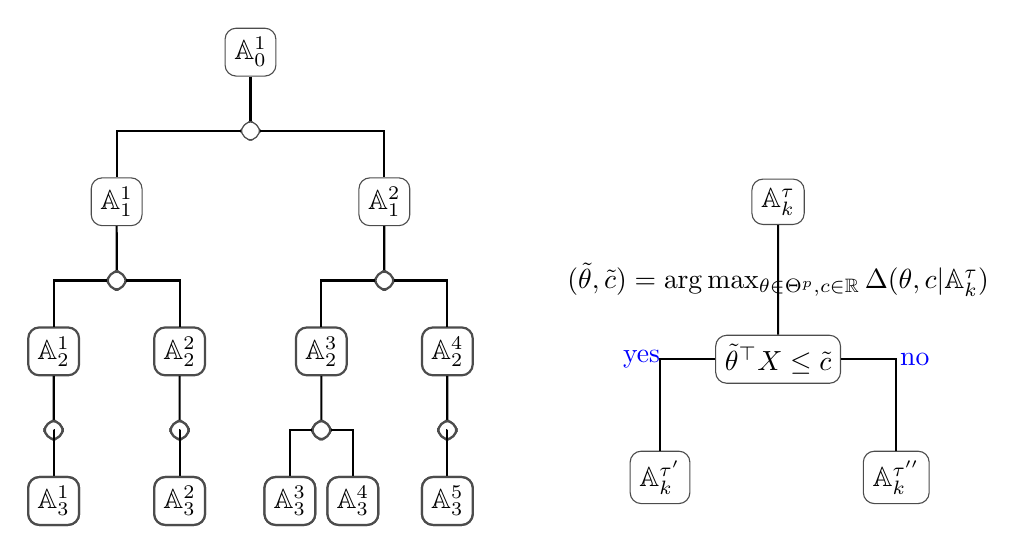
\begin{tikzpicture}[node distance=1cm,scale=0.6,
 	edge from parent/.style={black,thick,draw},
 	edge from parent path={(\tikzparentnode) -| (\tikzchildnode)}]

 	%ODT1
 	\node (S01) [process] {$\mathbb{A}_0^1$};
 	\node (N01) [process,below of=S01] {};
 	\draw [arrow] (S01) -- (N01);
 	\node (N01) [process,below of=S01] {}
 	child {
 		node (S11) [process,xshift=1cm] {$\mathbb{A}_1^1$};
 		\node (N11) [process,below of=S11] {};
 		\draw [arrow] (S11) -- (N11);
 		\node (N11) [process,below of=S11] {}
 		child {
 			node (S21) [process, xshift=1cm ] {$\mathbb{A}_2^1$};
 			\node (N21) [process,below of=S21] {};
 			\draw [arrow] (S21) -- (N21);
 			\node (N21) [process,below of=S21] {}
 			child {
 				node (S31) [process] {$\mathbb{A}_3^1$};
 				%\draw [arrow] (S33) -- ++(0,-1.5);
 				\node (S31) [process] {$\mathbb{A}_3^1$}
 			}
 			%			child {
 				%				node (S31) [process] {$\mathbb{A}_3^1$};
 				%				\node (S31) [process] {$\mathbb{A}_3^1$}
 				%			}
 			%			child [missing] {}
 			%			child {
 				%				node (S32) [process] {$\mathbb{A}_3^2$};
 				%				\node (S32) [process] {$\mathbb{A}_3^2$}
 				%			}
 		}
 		child [missing] {}
 		child [missing] {}
 		child [missing] {}
 		child {
 			node (S22) [process,xshift=-1cm] {$\mathbb{A}_2^2$};
 			\node (N22) [process,below of=S22] {};
 			\draw [arrow] (S22) -- (N22);
 			\node (N22) [process,below of=S22] {}
 			child {
 				node (S33) [process] {$\mathbb{A}_3^2$};
 				%\draw [arrow] (S33) -- ++(0,-1.5);
 				\node (S33) [process] {$\mathbb{A}_3^2$}
 			}
 		}
 	}
 	child [missing] {}
 	child [missing] {}
 	child [missing] {}
 	child [missing] {}
 	child [missing] {}
 	child {
 		node (S12) [process, xshift=-1cm] {$\mathbb{A}_1^2$};
 		\node (N12) [process,below of=S12] {};
 		\draw [arrow] (S12) -- (N12);
 		\node (N12) [process,below of=S12] {}
 		child {
 			node (S23) [process, xshift=1cm] {$\mathbb{A}_2^3$};
 			\node (N23) [process,below of=S23] {};
 			\draw [arrow] (S23) -- (N23);
 			\node (N23) [process,below of=S23] {}
 			child {
 				node (S34) [process, xshift=0.5cm] {$\mathbb{A}_3^3$};
 				%\draw [arrow] (S34) -- ++(0,-1.5);
 				\node (S34) [process, xshift=0.5cm] {$\mathbb{A}_3^3$}
 			}
 			child [missing] {}
 			child {
 				node (S35) [process, xshift=-0.5cm] {$\mathbb{A}_3^4$};
 				%\draw [arrow] (S35) -- ++(0,-1.5);
 				\node (S35) [process, xshift=-0.5cm] {$\mathbb{A}_3^4$}
 			}
 		}
 		child [missing] {}
 		child [missing] {}
 		child [missing] {}
 		child {
 			node (S24) [process, xshift=-1cm] {$\mathbb{A}_2^4$};
 			\node (N24) [process,below of=S24] {};
 			\draw [arrow] (S24) -- (N24);
 			\node (N24) [process,below of=S24] {}
 			child {
 				node (S36) [process] {$\mathbb{A}_3^5$};
 				%\draw [arrow] (S36) -- ++(0,-1.5);
 				\node (S36) [process] {$\mathbb{A}_3^5$}
 			}
 			%			child [missing] {}
 			% 			child {
 				% 				node (S37) [process] {$\mathbb{A}_3^7$};
 				% 				%\draw [arrow] (S37) -- ++(0,-1.5);
 				% 				\node (S37) [process] {$\mathbb{A}_3^7$}
 				% 			}
 		}
 	};


 	%ODT2
 	\node (input1) [process,right of=S12,xshift=4cm]{$\mathbb{A}_k^\tau$};
 	\node (decision1) [process,below of=input1,yshift=-1cm] {$ \tilde \theta^\top X  \leq \tilde c$};
 	\node (out1) [process,left of=decision1,xshift=-0.5cm,yshift=-1.5cm] {$\mathbb{A}_k^{\tau'}$};
 	\node (out2) [process,right of =decision1,xshift=0.5cm,yshift=-1.5cm]{$\mathbb{A}_k^{\tau''}$};

 	\draw [arrow] (input1) -- node {\bf $(\tilde \theta, \tilde c)=\mathop{\arg\max_{\theta\in\Theta^p, c\in\mathbb{R}}} {\Delta(\theta,c| \mathbb{A}_k^\tau)}$} (decision1);%\hspace{4.5cm}
 	%\draw [arrow] (decision1) -| node[above=0.1mm]{yes} (out1);
 	%\draw [arrow] (decision1) -| node[above=0.01mm]{no} (out2);
 	\draw [arrow] (decision1) -| node {\color{blue} yes  \ \ \ \ } (out1);%\Large
 	\draw [arrow] (decision1) -| node {\color{blue}\ \ \ \ no} (out2);%\Large
 \end{tikzpicture}
%}
\end{figure}


%\subsection{Estimation of the linear combination and ODT}

Thus, the main step in the ODT or ODRF is the estimation of the projection $ \theta $ or the selection of the linear combinations. Although many methods have been proposed, we find the projection pursuit regression is still the most efficient and is used in \pkg{ODRF}. The estimation is as follows. In any node $ \mathbb{A} $, define loss function
$$
 \Delta(\theta) =  \sum_{j=1}^q \sum_{X_i \in \mathbb{A}} \{y_{ij} - m_i(\theta^\top X_j)\}^2
$$
where  $ m_i $ is a nonparametric smoothing of the regression that minimizes  $\sum_{j=1}^b \{y_{ij} - m_i(\theta^\top X_j)\}^2$ with $ \theta $ given.  The nonparametric smoothing can be either the spline representation, or kernel smoothing, or the ``supsmu" of \pkg{ppr}.


\subsection{Build an ODRF }

\pkg{ODRF} builds the random forest in a slightly different ways from the existing forests. The detail is as follows.
Denote by $ X_{[q]} = (x_1', ..., x_q')$ a (random) subset of $ X  = (x_1, ..., x_p $ where $ q < p$ and $ \{x_1', ..., x_q'\} \subset \{x_1, ..., x_p\} $, and thus  by $X_{[q], r},\ r=1, 2, ...,$  a sequence of such subsets that may differ from one another.  In other words, with the same $ q $ and $ r$,  set $X_{[q], r}$ changes from place to place.
%Because given $q$ any element in $\Omega _q$ will be selected with equal probability, $\Omega $ is also a sample space equipped with probability
%$$\P(\S)=\frac{1}{p}\cdot\frac{1}{\binom{n}{Card(\S)}}$$
%for each $\S\subseteq \Omega $. Thus, $ \S_\tau, \tau\geq 1 $, can be regarded as a (random) sample of $ \Omega  $. Let $\Xi_{t_n-1}=(\S_1,\ldots, \S_{t_n-1})$  with  $t_n\geq 2$, which can be regarded as a random element in the product of probability spaces, $ \Omega  ^{\otimes t_n-1} $.
Using the idea of feature bagging, We first define $B$  random ODTs as follows.  %In Algorithm \ref{Algorithm.ODTtreereg}, we replace \textbf{lines 13-14} with following steps
%\begin{itemize}
%	\item For each node $A$, randomly choose $\S_\tau\in\Omega $ with  $Card(\S_\tau)=q$;
%	\item $(\hat{\theta}_{A},\hat{s}_A)=\argmax_{\theta_{\S_\tau}\in\Theta^q,s\in\mathbb{R}}{\Delta_{A,q}({\theta}_{\S_\tau},s)}$, where $\Delta_{A,q}$ is defined in the same way as $\Delta_{A}$ except that only  $\{(X_{i,\S_\tau},Y_i)\}_{i=1}^n$ are used in the calculation of $\Delta_{A,q}$;
%	\item Partition the node $A$ into $A^+_{\hat{\theta}_A,\hat{s}_A}=\{x\in A: \hat{\theta}_A^T\cdot x_{\S_\tau}\le \hat{s}_A\}$ and  $A^-_{\hat{\theta}_A,\hat{s}_A}=\{x\in A: \hat{\theta}_A^T\cdot x_{\S_\tau}> \hat{s}_A\}$.
%\end{itemize}
\begin{itemize}

  \item For each node $\mathbb{A}_k^\tau$, randomly select $q$, e.g. $INT(p/3)$, find variables $  X_{[q], r} = (x_1', ..., x_q') \subset X $, where $ r = 1, ..., R $ denotes $R$ random sets of variables.

  \item Find $$ \tilde \theta_{r} = arg \min_{\theta} \sum_{j=1}^q \sum_{X_i \in \mathbb{A}} \{y_{ij} - m_j(\theta^\top X_{[q],r, i})\}^2  $$
  where $ X_{[q],r, i} = (x_{i1}', ..., x_{iq}') $.
%  For each pair of $ \theta_{[q]},c_{(q)} $, define the partition
%  $$
%    \mathbb{A}_{k}^{\tau'} = \{ (X, y): X \in \mathbb{A}_k^\tau, \theta_{(q)}^\top X_{(q)}^r \le c_{(q)}\}, \ \
%    \mathbb{A}_{k}^{\tau''} = \{ (X, y): X \in \mathbb{A}_k^\tau, \theta_{(q)}^\top X_{(q)}^r > c_{(q)}\},
%  $$
%  $$
%  \Delta(\theta_{(q)},c_{(q)}, r| \mathbb{A}_k^\tau)= cov(Y|\mathbb{A}_k^\tau) - P(\mathbb{A}_k^{\tau'})cov(Y|\mathbb{A}_k^{\tau'}) - P(\mathbb{A}_k^{\tau''})cov(Y|\mathbb{A}_k^{\tau''})
%   $$
\item Define
  $$
    \mathbb{A}_{k,r}^{\tau'} = \{ X_i: X_i \in \mathbb{A}_k^\tau, \  \theta_{(q)}^\top X_{[q],r, i} \le c_{(q)}\}, \ \
    \mathbb{A}_{k,r}^{\tau''} = \{ X_i: X_i \in \mathbb{A}_k^\tau, \theta_{(q)}^\top X_{[q],r, i} > c_{(q)}\},
  $$
 \item  calculate
   $$
     (\tilde c_{(q)}, \tilde r) =arg  \min_{ c, r=1,..., R} \sum_{j=1}^q \sum_{X_i \in \mathbb{A}_{k,r}^{\tau'}} (y_{ij} - \bar y_{.j})^2  + \sum_{j=1}^q \sum_{X_i \in \mathbb{A}_{k, r}^{\tau''}} (y_{ij} - \bar y_{.j})^2.
   $$
 \item Split the node with $ (\tilde \theta_{\tilde r}, \tilde c_{\tilde r}, \tilde r) $, and the daughter nodes
\begin{center}
 $\mathbb{A}_{k+1}^{\tau'} = \mathbb{A}_{k+1,\tilde r}^{\tau'}$ and $\mathbb{A}_{k+1}^{\tau''} = \mathbb{A}_{k+1,\tilde r}^{\tau''}$.
\end{center}


  \item each tree produces one estimator $ \hat m_{n, b} (x) $

\end{itemize}
Finally, the ODR forest (ODRF) estimator is
  $$
    \hat m_{ODRF}(x) = B^{-1} \sum_{\tilde r=1}^B \hat m_{n, b} (x).
  $$


%% -- Illustrations ------------------------------------------------------------

%% - Virtually all JSS manuscripts list source code along with the generated
%%   output. The style files provide dedicated environments for this.
%% - In R, the environments {Sinput} and {Soutput} - as produced by Sweave() or
%%   or knitr using the render_sweave() hook - are used (without the need to
%%   load Sweave.sty).
%% - Equivalently, {CodeInput} and {CodeOutput} can be used.
%% - The code input should use "the usual" command prompt in the respective
%%   software system.
%% - For R code, the prompt "R> " should be used with "+  " as the
%%   continuation prompt.
%% - Comments within the code chunks should be avoided - these should be made
%%   within the regular LaTeX text.

%Implementation and application in practice
\section{Overview of the functions} \label{sec:functions}

 In this section, we introduce \pkg{ODRF} package main function implementation in \proglang{R}. We use some \proglang{R}'s \code{S3} method, including the base \proglang{R} functions \fct{print}, \fct{predict} and \fct{plot} in the \pkg{base} \citep{R} package, the transform function \fct{as.part} in the \pkg{partykit} \citep{2015Partykit} package and our self-defined functions  \fct{ODT}, \fct{ODRF}, \fct{online}, \fct{prune} in the \pkg{ODRF} package. In the \pkg{ODRF} package, the function \fct{best.cut.node} to find the optimal split variables and split nodes and the projection pursuit function \fct{PPO} to estimate the projection direction. They both make \proglang{R} interact with \proglang{C++} by the \pkg{Rcpp} package, which greatly speeds up the the computation time to our program. The details of the function usage are described below.
\subsection[print the tree structure of ODT and the estimation error of ODRF]{\code{print} the tree structure of \code{ODT} and the estimation error of \code{ODRF}}
Functions \fct{ODT} and \fct{ODRF} are the two main functions of the \pkg{ODRF} package, \fct{ODRF} is ODT-based random forests. They can both be used for classification and regression and are similar in usage. We provide two data input ways for these two \code{S3} methods.

The first way is \code{formula = y ~ .,data = data.frame(X, y = y)} or \code{formula = y ~ X} with class \code{formula}, and usage are
\begin{Code}
## S3 method for class 'formula'
ODT(formula, data = NULL, type = "auto", NodeRotateFun = "RotMatPPO",
  FunDir = getwd(), paramList =NULL, MaxDepth = Inf, numNode = Inf,
  MinLeaf = 5, Levels = NULL, subset = NULL, weights = NULL,
  na.action = na.fail, catLabel = NULL, Xcat = 0, Xscale = "Min-max",
  TreeRandRotate = FALSE, ...)
ODRF(formula, data = NULL, type = "auto", NodeRotateFun = "RotMatPPO",
  FunDir = getwd(), paramList = NULL, ntrees = 100, storeOOB = TRUE,
  replacement = TRUE, stratify = TRUE, numOOB = 1/3, parallel = TRUE,
  numCores = Inf, seed = 220924, MaxDepth = Inf, numNode = Inf,
  MinLeaf = 5, subset = NULL, weights = NULL, na.action = na.fail,
  catLabel = NULL, Xcat = 0, Xscale = "Min-max", TreeRandRotate = FALSE, ...)
\end{Code}
The second way is \code{X = X, y = y} with class \code{default}, and usage are
\begin{Code}
## Default S3 method:
ODT(X, y, type = "auto", NodeRotateFun = "RotMatPPO", ...)
ODRF(X, y, type = "auto", NodeRotateFun = "RotMatPPO", ...)
\end{Code}
Arguments
\begin{itemize}
	\item \code{type}: The criterion used for splitting the nodes, 'i-classification': information gain and 'g-classification': gini impurity index for classification, 'regression': mean square error for regression. 'auto' (default): If the response in data or y is a factor, 'g-classification' is used, otherwise regression is assumed.(see \code{?best.cut.node})
	\item \code{NodeRotateFun}: Name of the function of class character that implements a linear combination of predictors in the split node. Default is \code{"RotMatPPO"} with \code{model = "PPR"} (see \code{?RotMatPPO}). Users can define this function, for details see \code{?RotMatMake}.
	\item \code{catLabel}: A category labels of class \code{list} in predictors. (default NULL, for details see the following examples)
	\item \code{other arguments}: Other arguments we do not introduce here, users can see \code{?ODT} and \code{?ODRF}. These arguments are defaulted to the optimal values, so that the user does not need to modify them except for special needs.
\end{itemize}
where \code{formula} plus \code{data} is the now standard way of specifying relationships in \proglang{R}. The remaining arguments in the first line (\code{subset}, \code{na.action}, and \code{weights}) are also standard for setting up formula-based models in \proglang{R}.

Before classification or regression, it is necessary to do some pre-processing to the data. In addition to the standard arguments \code{subset}, \code{na.action}, and \code{weights}, we also provide \code{Xscale} for the predictors to be normalized. Any feature $x$ of predictor $X$ were scaled to $[0,1]$ using the maximal or quantile value of the in-sample, that is $\frac{x-x_{L}}{x_{U}-x_{L}}$.
%\begin{equation} \label{eq:scale}
	%\frac{x-x_{L}}{x_{U}-x_{L}}.
%\end{equation}
Where $x_{U}$ and $x_{L}$ denote the upper and lower bounds of $x$, respectively. When using minima (defaulte \code{Xscale = "Min-max"}), $x_{U}$ = \code{max(x)}, $x_{L}$ = \code{min(x)}, when using quantile (\code{Xscale = "Quantile"}), $x_{U}$ = \code{quantile(x, 0.95)}, $x_{L}$ = \code{quantile(x, 0.05)}.
Sometimes the predictor $X$ has category variables that must be transformed into dummy variables. The arguments \code{catLabel} and \code{Xcat} in our program can automatically deal with category variables. The user can enter the ordinal number of the category variable with \code{Xcat} and let \code{catLabel = NULL}. It even is allowed to let \code{Xcat = NULL}, we will use the condition \code{(length( unique( x )) < 10) \& (n > 20)} to judge which one is the category variable, and for details see examples of \code{ODT} or \code{ODRF}.%The example is as follows.
%
Print the tree structure of class \code{ODT} and \code{party}, and the model estimation error of class \code{ODRF}.
%
\begin{Schunk}
\begin{Sinput}
R> data(iris, package = "datasets")
R> tree <- ODT(Species ~ ., data = iris)
R> tree
\end{Sinput}
\begin{Soutput}
============================================================= 
Oblique Classification Tree structure 
=============================================================

1) root
   node2)# proj1*X < 0.29 -> (leaf1 = setosa)
   node3)  proj1*X >= 0.29
      node4)  proj2*X < 0.69
         node6)# proj3*X < 0.58 -> (leaf2 = versicolor)
         node7)  proj3*X >= 0.58
            node10)# proj5*X < 0.35 -> (leaf5 = versicolor)
            node11)# proj5*X >= 0.35 -> (leaf6 = versicolor)
      node5)  proj2*X >= 0.69
         node8)# proj4*X < 0.54 -> (leaf3 = virginica)
         node9)# proj4*X >= 0.54 -> (leaf4 = virginica)
\end{Soutput}
\begin{Sinput}
R> party.tree <- as.party(tree, data = iris)
R> party.tree
\end{Sinput}
\begin{Soutput}
Model formula:
Species ~ Sepal.Length + Sepal.Width + Petal.Length + Petal.Width

Fitted party:
[1] root
|   [2] proj1X >= 0.29167
|   |   [3] proj2X >= 0.6875
|   |   |   [4] proj4X >= 0.54167: virginica (n = 35, err = 0.0%)
|   |   |   [5] proj4X < 0.54167: virginica (n = 11, err = 9.1%)
|   |   [6] proj2X < 0.6875
|   |   |   [7] proj3X >= 0.58475
|   |   |   |   [8] proj5X >= 0.35417: versicolor (n = 14, err = 7.1%)
|   |   |   |   [9] proj5X < 0.35417: versicolor (n = 11, err = 36.4%)
|   |   |   [10] proj3X < 0.58475: versicolor (n = 29, err = 0.0%)
|   [11] proj1X < 0.29167: setosa (n = 50, err = 0.0%)

Number of inner nodes:    5
Number of terminal nodes: 6
\end{Soutput}
\begin{Sinput}
R> forest <- ODRF(Species ~ ., data = iris, parallel = FALSE)
R> forest
\end{Sinput}
\begin{Soutput}
Call:
 ODRF.formula(formula = Species ~ ., data = data, parallel = FALSE) 
               Type of oblique decision random forest: classification
                                      Number of trees: 100
                           OOB estimate of error rate: 6%
Confusion matrix:
           setosa versicolor virginica class_error
setosa         50          0         0  0.00000000
versicolor      0         46         5  0.09803902
virginica       0          4        45  0.08163249
\end{Soutput}
\end{Schunk}
\fct{print} is \proglang{R}'s standard \code{S3} method used to print the results of various objects of class. We use a similar way to \fct{print} in \pkg{PPtreeViz} package \cite{lee2018pptreeviz} to print the tree structure of \fct{ODT}, which shows each node partition of \code{ODT} in detail. When the options \code{projection = TRUE, cutvalue = TRUE} denotes to print projection coefficient and cutoff values in each node respectively. Currently, the \pkg{partykit} package is commonly used to summarize and vi-sualize tree structure in various ways. The function \fct{as.party} in \pkg{partykit} package can convert the trees in other \proglang{R} packages to \code{party} class. We define the \fct{as.party.ODT} function to add \code{ODT} class to the \code{party} class, so that we can use the same function \fct{print} to print the tree structure of the \code{party} class. In addition, we can also use the function \fct{print} to print the model estimation error for the class \fct{ODRF}.
\subsection[Classification and regression with ODT and ODRF]{Classification and regression with functions \fct{ODT} and \fct{ODRF}}
\fct{predict} is the standard \code{S3} method used to predict new data for various objects of class. we defined the functions \fct{predict.ODT} and \fct{predict.ODRF} to predict \code{Xnew} for classes \fct{ODT} and \fct{ODRF} respectively. The default output of \fct{predict} is \code{response} which is the prediced values of the new data. When the argument \code{leafnode = TRUE} in \fct{predict.ODT}, outputs the leaf node sequence number that the new data is partitioned, and it can be used for clustering the data. \fct{predict.ODT} also provides options \code{type} and \code{weight.tree} to denote the output type and whether to weight the tree respectively, see \code{?predict.ODRF} for details.
\begin{Code}
## S3 method for class 'ODT'
predict(ppTree, Xnew, leafnode = FALSE)
## S3 method for class 'ODRF'
predict(ppForest, Xnew, type = "response", weight.tree = FALSE)
\end{Code}
We also defined \code{S3} methods \code{online} and \code{prune} used to online structure training and estimation error pruning for classes \code{ODT} and \code{ODRF}, respectively, and they can significantly improve the model accuracy. \code{online} Update existing \code{ODT} and \code{ODRF} using batches of data. \code{prune} is judged to prune or not based on whether the error of computing new data is reduced or not, and our pruning begins from the last leaf node. For class \code{ODRF}, let \code{prune}'s argument \code{useOOB=TRUE} to use 'out-of-bag' for pruning.
\begin{Code}
## S3 method for class 'ODT' and 'ODRF'
online(obj, X = NULL, y = NULL, weights = NULL, ...)
## S3 method for class 'ODT'
prune(ppTree, X, y, MaxDepth = 1, ...)
## S3 method for class 'ODRF'
prune(ppForest, X, y, MaxDepth = 1, useOOB = TRUE, ...)
\end{Code}
%
Classification and regression with \fct{ODRF} and \fct{ODT} respectively, and the model is trained with \fct{online} and prune with \fct{prune}, respectively.
%
\begin{Schunk}
\begin{Sinput}
R> data(seeds, package = "ODRF")
R> set.seed(18)
R> train <- sample(1:209, 120)
R> train_data <- data.frame(seeds[train, ])
R> test_data <- data.frame(seeds[-train, ])
R> index <- seq(floor(nrow(train_data) / 2))
R> forest <- ODRF(varieties_of_wheat ~ ., train_data,
+    type = "i-classification", parallel = FALSE
+  )
R> pred <- predict(forest, test_data[, -8])
R> e.forest <- mean(pred != test_data[, 8])
R> forest1 <- ODRF(varieties_of_wheat ~ ., train_data[index, ],
+    type = "i-classification", parallel = FALSE
+  )
R> pred <- predict(forest1, test_data[, -8])
R> e.forest.1 <- mean(pred != test_data[, 8])
R> forest2 <- ODRF(varieties_of_wheat ~ ., train_data[-index, ],
+    type = "i-classification", parallel = FALSE
+  )
R> pred <- predict(forest2, test_data[, -8])
R> e.forest.2 <- mean(pred != test_data[, 8])
R> forest.online <- online(
+    forest1, train_data[-index, -8],
+    train_data[-index, 8]
+  )
R> pred <- predict(forest.online, test_data[, -8])
R> e.forest.online <- mean(pred != test_data[, 8])
R> forest.prune <- prune(forest1, train_data[-index, -8],
+    train_data[-index, 8],
+    useOOB = FALSE
+  )
R> pred <- predict(forest.prune, test_data[, -8])
R> e.forest.prune <- mean(pred != test_data[, 8])
R> print(c(
+    forest = e.forest, forest1 = e.forest.1, forest2 = e.forest.2,
+    forest.online = e.forest.online, forest.prune = e.forest.prune
+  ))
\end{Sinput}
\begin{Soutput}
       forest       forest1       forest2 forest.online  forest.prune 
   0.04494382    0.07865169    0.08988764    0.06741573    0.07865169 
\end{Soutput}
\begin{Sinput}
R> data(body_fat, package = "ODRF")
R> set.seed(9)
R> train <- sample(1:252, 120)
R> train_data <- data.frame(body_fat[train, ])
R> test_data <- data.frame(body_fat[-train, ])
R> index <- seq(floor(nrow(train_data) / 2))
R> tree <- ODT(Density ~ ., train_data, type = "regression")
R> pred <- predict(tree, test_data[, -1])
R> e.tree <- mean((pred - test_data[, 1])^2)
R> tree1 <- ODT(Density ~ ., train_data[index, ], type = "regression")
R> pred <- predict(tree1, test_data[, -1])
R> e.tree.1 <- mean((pred - test_data[, 1])^2)
R> tree2 <- ODT(Density ~ ., train_data[-index, ], type = "regression")
R> pred <- predict(tree2, test_data[, -1])
R> e.tree.2 <- mean((pred - test_data[, 1])^2)
R> tree.online <- online(tree1, train_data[-index, -1], train_data[-index, 1])
R> pred <- predict(tree.online, test_data[, -1])
R> e.tree.online <- mean((pred - test_data[, 1])^2)
R> tree.prune <- prune(tree1, train_data[-index, -1], train_data[-index, 1])
R> pred <- predict(tree.prune, test_data[, -1])
R> e.tree.prune <- mean((pred - test_data[, 1])^2)
R> print(c(
+    tree = e.tree, tree1 = e.tree.1, tree2 = e.tree.2,
+    tree.online = e.tree.online, tree.prune = e.tree.prune
+  ))
\end{Sinput}
\begin{Soutput}
        tree        tree1        tree2  tree.online   tree.prune 
3.428481e-05 3.614067e-05 5.093495e-05 3.626432e-05 3.614067e-05 
\end{Soutput}
\end{Schunk}
As shown in the classification and regression results above, the training data \code{train_data} is divided into two batches equally, then the first batch is used to train \code{ODT} and \code{ODRF}, and the second batch is used to update the model by \fct{online}. The error after the model update is significantly smaller than that of one batch of data alone, and the model is also pruned by \fct{prune} and the same effect is achieved.

\subsection[Create a projection matrix with the RotMat* function]{Create a projection matrix with the \code{RotMat*} function}
We provide the functions \fct{RotMatPPO}, \fct{RotMatRand} and \fct{RotMatRF} for creating rotation matrix by projection pursuit optimization model (\emph{PPO}) \cite{cook2008grand}, same random rotation as \fct{RandMatBinary} in \pkg{rerf} package and single feature similar to random forest, respectively. The function \fct{PPO} is to find the best projection using various projectin pursuit models, including \code{"PPR"} (default): projection projection regression from \fct{ppr} in \pkg{stats} package \cite{friedman1981projection}, \code{"Log"}: logistic based on \fct{nnet} in \pkg{nnet} package \cite{nnet}, \code{"Rand"}: The random projection generated from $\{-1, 1\}$, argument \code{PPmethod} of function \fct{PPopt} in \pkg{PPtreeViz} package, and argument \code{findex} of function \fct{PP\_Optimizer} in \pkg{Pursuit} package \cite{Pursuit}. Note that \pkg{PPtreeViz} and \pkg{Pursuit} are only available for classification. The generated rotation matrix has three columns, the first column (\code{Variable}). Variable to be projected, the second column (\code{Number}): Number of projections, and the third column (\code{Coefficient}): the coefficient of the projected matrix. In addition, the user can define a projection matrix function, see the \pkg{ODRF} help file for more details on usage.%,We provide a several examples as follows, just let the argument \code{RotMatFun} be the name of the defined function and let the argument \code{paramList} be the arguments used in the defined function, or use the function \fct{RotMatMake} to define the projection matrix by the following way.
\begin{Code}
RotMatPPO(X,y,model = "PPR",type = "i-classification",weights = NULL,
  dimProj,numProj,catLabel = NULL, ...)
RotMatRand(dimX,randDist = "Binary",numProj = ceiling(sqrt(dimX)),
  dimProj = "Rand",sparsity, prob = 0.5,lambda = 1,catLabel = NULL,...)
RotMatRF(dimX, numProj, catLabel = NULL, ...)
RotMatMake(X = NULL,y = NULL,RotMatFun = "RotMatPPO",PPFun = "PPO",
  FunDir = getwd(),paramList = NULL, ...)
PPO(X, y, model = "PPR", type = "i-classification", weights = NULL
\end{Code}
%
To show that \fct{PPO} with different \code{model} to do classification and regression and used to \fct{RotMatPPO}. after that show simple usage of functions \fct{RotMatRand} and \fct{RotMatRF}.% Finally explain how to define the projection matrix function and train \code{ODT} by two ways.
%
\begin{Schunk}
\begin{Sinput}
R> data(seeds, package = "ODRF")
R> (PP <- PPO(seeds[, 1:7], seeds[, 8], model = "LDA", type = "i-classification"))
\end{Sinput}
\begin{Soutput}
[1]  0.59669228  0.62575666 -0.47202518  0.03032322  0.01598554
[6] -0.14782205 -0.08094918
\end{Soutput}
\begin{Sinput}
R> RotMat <- RotMatPPO(seeds[, 1:7], seeds[, 8],
+    model = "Log",
+    type = "i-classification"
+  )
R> head(RotMat)
\end{Sinput}
\begin{Soutput}
     Variable Number Coefficient
[1,]        7      1   1.0000000
[2,]        3      2   1.0000000
[3,]        2      3   1.0000000
[4,]        1      4  -0.8635696
[5,]        5      4   0.5042297
[6,]        3      5   1.0000000
\end{Soutput}
\begin{Sinput}
R> data(body_fat, package = "ODRF")
R> (PP <- PPO(body_fat[, 2:15], body_fat[, 1], model = "Log", type = "regression"))
\end{Sinput}
\begin{Soutput}
 [1]  0.0500396390 -0.0004203160  0.0017394832 -0.0038324798
 [5] -0.0035428671 -0.0036891205  0.0033979058 -0.0057153924
 [9]  0.0002710173 -0.0043282445  0.0044730880  0.0029504953
[13] -0.0004124229 -0.0172101483
\end{Soutput}
\begin{Sinput}
R> RotMat <- RotMatPPO(seeds[, 1:7], seeds[, 8],
+    model = "PPR",
+    type = "i-classification"
+  )
R> head(RotMat)
\end{Sinput}
\begin{Soutput}
     Variable Number Coefficient
[1,]        3      1  1.00000000
[2,]        6      2  1.00000000
[3,]        4      3  1.00000000
[4,]        3      4 -0.99619128
[5,]        2      4 -0.08719482
[6,]        1      5  1.00000000
\end{Soutput}
\begin{Sinput}
R> set.seed(22)
R> X <- matrix(rnorm(1000), 100, 10)
R> y <- (rnorm(100) > 0) + 0
R> paramList <- list(dimX = 8, numProj = 3, sparsity = 0.25, prob = 0.5)
R> (RotMat <- do.call(RotMatRand, paramList))
\end{Sinput}
\begin{Soutput}
     Variable Number Coefficient
[1,]        7      1           1
[2,]        4      2          -1
[3,]        5      2           1
[4,]        6      2           1
[5,]        7      2           1
[6,]        8      3          -1
\end{Soutput}
\begin{Sinput}
R> paramList <- list(dimX = 8, numProj = 3, catLabel = NULL)
R> (RotMat <- do.call(RotMatRF, paramList))
\end{Sinput}
\begin{Soutput}
     Variable Number Coefficient
[1,]        6      1           1
[2,]        7      2           1
[3,]        5      3           1
\end{Soutput}
\end{Schunk}

\section{Real examples} \label{sec:examples}
In this section, we compare ODT with other axis-aligned and oblique tree methods in a more rigorous benchmark comparison. the tree algorithms are compared on 52 real data sets with continuous and categorical response. In addition, we add the forest methods and consider the time consumption and tree complexity. The rest of the section describes how to use our ODRF package in real data, and we explain the use of two data sets with continuous and categorical response.

\subsection{Performance comparison}
we follow the experimental design of \cite{zhan2022consistency}, where we show the performance of  \code{ODRF}, but in this article we show the performance of \code{ODT}. We use 26 real data sets with continuous responses  and 26 data sets with categorical response for regression prediction and classification respectively. Where the data set has categorical responses, seeds, breast tissue and waveforms dataset are triple, six and triple category responses respectively, and all other data are binary category responses (0 and 1). Our data are mainly obtained from the UCI machine learning database (A) \url{https://archive.ics.uci.edu/ml/datasets}, the kaggle database (B) \url{https://www.kaggle.com}, and Rainforth and Wood \cite{rainforth2015canonical} Collection Datasets (C) \url{https://github.com/twgr/ccfs/}.
If there are any missing values in a data, the corresponding samples are removed from the data. In the calculation, Each predictor is scaled to [0, 1] using the minima method of Section \ref{sec:print} proposed.

We compare two different random rotation oblique tree methods, Blaser and Fryzlewicz\cite{blaser2016random} proposed the Random Rotation Random Forest (\emph{RotRF}), and Tomita et al.\cite{tomita2020sparse} proposed Sparse Projection Oblique Randomer Forests (\emph{SPORF}). Note that, SPORF unlike RotRF, the random rotation in SPORF is carried out at separately each node, as opposed to using a single rotation for the whole tree. We use single trees and denote as \emph{RotT} and \emph{SPOT} respectively, and we use function \fct{ODT} in \pkg{ODRF} package to implement RotT and  SPOT. In additition, there are two oblique decision tree methods used for classification, projection pursuit classification trees (PPT) \cite{lee2018pptreeviz} with function \fct{PPTreeclass} in \pkg{PPtreeViz} package and Oblique Trees for Classification Data (OT)  \cite{truong2009fast} with function \fct{oblique.tree} in \pkg{oblique.tree} package. To show the performance of ODT, we also compare four axis-aligned tree methods  in Section \ref{sec:intro}, including \emph{CART} with function \fct{rpart} in \pkg{rpart} package, \emph{ERT} with function \fct{RLT} in \pkg{RLT} package, \emph{EVT} with function \fct{evtree} in \pkg{evtree} package, and \emph{CT} with function \fct{ctree} in \pkg{partykit} package.
	For all the R functions  and  packages, their default values of tuning parameters are used. Note that because \emph{PPT} and \emph{OT} cannot do the regression, we only report the classification results. In order to improve speed, this portion of code was implemented in C++ and integrated into R using the Rcpp package. Further speedup is achieved through multicore parallelization of tree construction and byte-compilation via the R compiler package.%\cite{tomita2020sparse}.

For each data set, we randomly partition it into training set and test set. The training set consists of $n=\min(\lfloor 2N/3\rfloor,2000)$ randomly selected observations, where $N$ is the number of observations in the original data sets, and the remaining observations form the test set. For regression, the relative prediction error, defined as
$$RPE=\sum_{i\in \text{test set}}(\hat{y}_i-y_i)^2/\sum_{i\in \text{test set}}(\bar{y}_{\text{train}}-y_i)^2,$$
where $\bar{y}_{\text{train}}$ is naive predictions based on the average of $y$ in the training sets, is used to measure the performance of a method. For classification, the misclassification rate, defined as
$$MR=\sum_{i\in \text{test set}} 1(\hat{y}_i \neq y_i) /(N-n),$$
is used to measure the performance. For each data set, the random partition is repeated 100 times,  and averages of the RPEs or MRs are calculated to compare different methods. The calculation results are listed in Table~\ref{Table1} and Table~\ref{Table2}. The smallest RPE or MR for each data set is highlighted in \textbf{bold} font.

\begin{table}[t!]
\centering
%\begin{center}
\begin{minipage}{\textwidth}
\setlength{\tabcolsep}{1.0mm}{
  \begin{tabular}{@{\extracolsep{\fill}}lrrccccccc@{\extracolsep{\fill}}}%{lrrrrrrrrr}% {\textwidth}{@{\extracolsep{\fill}}lrrrrrrrrr@{\extracolsep{\fill}}}%{lrrrrrrrrr{7.4cm}}%
    %\multirow{2}[4]{*}{Dataset} & \multirow{2}[4]{*}{n} & \multirow{2}[4]{*}{p} & \multicolumn{4}{c}{Axis-aligned} & \multicolumn{3}{c}{Oblique} \\
  %\cmidrule{4-10}          &       &       & CART  & ERT   & EVT   & CT    & rotT  & SPOT  & ODT \\
  \toprule%
  &       &         & \multicolumn{4}{c}{Axis-aligned} & \multicolumn{3}{c}{Oblique} \\
  %\cline{4-7} \cline{8-10}
  \cmidrule(lr){4-7}\cmidrule(lr){8-10}%
  Dataset&   n    &   p      & CART  & ERT   & EVT   & CT    & RotT  & SPOT  & ODT \\
  \midrule
  Servo (C) & 166   & 4     & 0.298  & 0.871  & \pmb{0.246} & 0.300  & 0.673  & 0.406  & 0.256  \\
  Auto MPG (C) & 391   & 7     & 0.213  & 0.318  & 0.221  & 0.192  & 0.237  & 0.235  & \pmb{0.185} \\
  Concrete Compressive Strength (A) & 1030  & 8     & 0.314  & 0.501  & 0.307  & 0.248  & 0.453  & 0.357  & \pmb{0.189} \\
  Boston house price (A) & 506   & 13    & 0.275  & 0.444  & 0.293  & 0.275  & 0.427  & 0.358  & \pmb{0.256} \\
  Wild blueberry yield (B) & 777   & 13    & 0.228  & 0.329  & 0.225  & 0.189  & 0.262  & 0.199  & \pmb{0.098} \\
  Body fat (B) & 252   & 14    & 0.073  & 0.442  & 0.084  & 0.061  & 0.401  & 0.353  & \pmb{0.059} \\
  Paris housing price (B) & 10000 & 16    & 0.018  & 0.284  & 0.004  & \pmb{0.000} & 0.681  & 0.435  & \pmb{0.000} \\
  House sales in King County (B) & 21613 & 18    & 0.326  & 0.425  & 0.292  & 0.256  & 0.388  & 0.314  & \pmb{0.254} \\
  Bar crawl (B) & 7590  & 21    & 0.318  & 0.416  & 0.303  & \pmb{0.268} & 0.464  & 0.370  & \pmb{0.268} \\
  Auto 93 (C) & 81    & 22    & 0.620  & 0.967  & 0.697  & 0.602  & 0.778  & 0.702  & \pmb{0.543} \\
  Auto horsepower (C) & 159   & 24    & 0.236  & 0.347  & 0.251  & 0.238  & 0.448  & 0.325  & \pmb{0.186} \\
  Wave Energy Converters (A) & 71998 & 32    & 0.543  & 0.717  & 0.557  & \pmb{0.488} & 0.544  & 0.534  & 0.547  \\
  Sidney house price (B) & 30000 & 37    & 0.703  & 1.040  & 0.705  & \pmb{0.646} & 0.803  & 0.737  & 0.720  \\
  Facebook comment volume (A) & 18370 & 52    & 0.630  & 1.134  & 0.676  & \pmb{0.620} & 0.985  & 0.843  & 0.708  \\
  Baseball player statistics (B) & 4535  & 74    & 0.039  & 0.162  & 0.013  & 0.008  & 0.631  & 0.433  & \pmb{0.003} \\
  Gold price prediction (B) & 1718  & 74    & 0.042  & 0.020  & 0.021  & 0.014  & 0.109  & 0.021  & \pmb{0.010} \\
  CNNpred (A) & 1441  & 76    & 0.032  & 0.016  & 0.011  & 0.003  & 0.119  & 0.065  & \pmb{0.002} \\
  Warsaw flat rent price (B) & 3472  & 78    & 0.433  & 0.678  & 0.424  & \pmb{0.398} & 1.019  & 0.565  & 0.498  \\
  Superconductivity (A) & 21263 & 81    & 0.284  & 0.319  & 0.263  & 0.241  & 0.280  & 0.253  & \pmb{0.240} \\
  Buzz in social media (A) & 28179 & 96    & 0.140  & 0.252  & 0.198  & \pmb{0.126} & 0.292  & 0.219  & 0.196  \\
  Communities and Crime (A) & 1994  & 101   & 0.460  & 0.720  & 0.467  & \pmb{0.434} & 0.604  & 0.561  & 0.614  \\
  Residential building-Sales (A) & 372   & 103   & 0.060  & 0.243  & 0.060  & \pmb{0.040} & 0.330  & 0.267  & \pmb{0.040} \\
  Residential building-Cost (A) & 372   & 103   & 0.111  & 0.212  & 0.129  & 0.094  & 0.241  & 0.204  & \pmb{0.086} \\
  Credit score (B) & 80000 & 259   & 0.274  & 0.299  & 0.269  & \pmb{0.234} & 0.490  & 0.267  & 0.236  \\
  CT slices (A) & 53500 & 380   & 0.224  & 0.209  & 0.238  & 0.187  & 0.374  & 0.225  & \pmb{0.154} \\
  UJIndoor-Longitude (A) & 19937 & 465   & 0.087  & 0.101  & 0.140  & 0.064  & 0.198  & 0.054  & \pmb{0.026} \\
  \hline
  \multicolumn{3}{c}{Average RPE(\%) across all data sets}&   0.269  & 0.441  & 0.273  & 0.239  & 0.470  & 0.358  & 0.245  \\
  \multicolumn{3}{c}{no. of bests in 26 datasets} &0     & 0     & 1     & 10    & 0     & 0     & 18  \\
  \bottomrule
  \end{tabular}}
\end{minipage}
%	\end{center}
\caption{Regression: average RPE based on 100 random partitions of each data set into training and test sets}\label{Table1}%
\end{table}

\begin{table}[t!]
\centering
%\begin{center}
\begin{minipage}{\textwidth}
\setlength{\tabcolsep}{0.05mm}{
  \begin{tabular}{@{\extracolsep{\fill}}lrrrrrrrrrrr@{\extracolsep{\fill}}}%{lrrrrrrrrr}% {\textwidth}{@{\extracolsep{\fill}}lrrrrrrrrr@{\extracolsep{\fill}}}%{lrrrrrrrrr{7.4cm}}%
    %\multirow{2}[4]{*}{Dataset} & \multirow{2}[4]{*}{n} & \multirow{2}[4]{*}{p} & \multicolumn{4}{c}{Axis-aligned} & \multicolumn{3}{c}{Oblique} \\
  %\cmidrule{4-10}          &       &       & CART  & ERT   & EVT   & CT    & rotT  & SPOT  & ODT \\
  \toprule%
  &       &         & \multicolumn{4}{c}{Axis-aligned} & \multicolumn{5}{c}{Oblique} \\
  %\cline{4-7} \cline{8-10}
  \cmidrule(lr){4-7}\cmidrule(lr){8-12}%
  Dataset&   n    &   p      & CART  & ERT   & EVT   & CT    & RotT  & SPOT  &PPT & OT & ODT \\
  \midrule
  Seeds (C) & 210   & 7     & 9.66  & 95.59  & 10.89  & 12.39  & 10.87  & 11.56  & \pmb{4.27} & 5.30  & 7.21  \\
  Breast tissue (C)  & 106   & 9     & 36.25  & 91.90  & 38.78  & 42.62  & 41.90  & 39.94  & \pmb{33.63} & 39.14  & 36.67  \\
  MAGIC Gamma telescope (A) & 19020 & 10    & 17.83  & 25.17  & 18.44  & \pmb{17.79} & 22.74  & 21.73  & 20.69  & 18.88  & 19.84  \\
  Indian liver patient (A) & 579   & 10    & 32.01  & 33.67  & 30.56  & \pmb{29.64} & 34.46  & 32.91  & 37.30  & 33.49  & 33.30  \\
  Heart disease (A) & 270   & 13    & 21.91  & 27.20  & 23.18  & 25.28  & 27.20  & 25.91  & \pmb{16.20} & 23.61  & 24.09  \\
  EEG eye state (A) & 14980 & 14    & 29.34  & 33.18  & 28.92  & 32.38  & 28.81  & 26.55  & 37.75  & 23.89  & \pmb{22.30} \\
  seismic-bumps (A) & 2584  & 15    & 7.05  & 9.17  & \pmb{6.56} & 6.62  & 9.50  & 9.94  & 18.31  & 10.18  & 10.54  \\
  Retinopathy debrecen (A) & 1151  & 19    & 35.89  & 40.03  & 35.48  & 37.03  & 39.13  & 36.59  & \pmb{29.37} & 32.66  & 31.84  \\
  Waveform (C)  & 5000  & 21    & 26.36  & 91.06  & 25.29  & 24.72  & 26.63  & 26.57  & 21.95  & \pmb{19.08} & 20.24  \\
  Parkinson multiple sound (B) & 1208  & 26    & \pmb{34.39} & 38.82  & 34.89  & 37.10  & 36.44  & 35.50  & 35.23  & 36.88  & 35.18  \\
  Pistachio (B) & 2148  & 28    & 13.62  & 17.29  & 13.75  & 13.67  & 16.41  & 15.63  & \pmb{11.55} & 11.75  & 12.52  \\
  Breast cancer (B) & 569   & 30    & 7.07  & 9.37  & 6.74  & 6.34  & 7.66  & 7.06  & \pmb{4.41} & 6.16  & 5.32  \\
  Ionosphere (A) & 351   & 33    & 12.40  & 17.84  & 11.52  & \pmb{10.22} & 15.27  & 13.56  & 13.92  & 16.26  & 12.40  \\
  QSAR biodegradation (A) & 1055  & 41    & 17.88  & 20.84  & 18.30  & 19.65  & 20.60  & 19.41  & \pmb{15.52} & 19.60  & 18.26  \\
  Spambase (A) & 4601  & 57    & 10.57  & 11.27  & 9.82  & 10.49  & 16.49  & 10.96  & 9.75  & 10.14  & \pmb{8.88} \\
  Mice protein expression (A) & 1047  & 70    & 13.60  & 17.63  & 16.87  & 13.93  & 16.42  & 14.04  & \pmb{3.58} & 4.62  & 5.70  \\
  Ozone level detection (A) & 1847  & 72    & 8.02  & 9.94  & \pmb{6.89} & 7.51  & 9.47  & 9.40  & 19.55  & 11.53  & 9.99  \\
  Company bankruptcy (B) & 6819  & 94    & 3.82  & 4.71  & \pmb{3.25} & 3.44  & 5.16  & 4.65  & 17.13  & 7.02  & 5.41  \\
  Hill valley noisy (C) & 1212  & 100   & 47.52  & 75.83  & 49.07  & 51.75  & 40.61  & 38.54  & 33.63  & 20.95  & \pmb{18.27} \\
  Hill valley (C) & 1212  & 100   & 48.22  & 46.38  & 48.29  & 51.41  & 30.87  & 10.23  & 29.90  & 13.95  & \pmb{0.04} \\
  Musk (A) & 6598  & 166   & 6.82  & 9.87  & 10.03  & 7.46  & 10.01  & 8.40  & \pmb{6.75} & 8.55  & 8.32  \\
  ECG heartbeat (B) & 14550 & 186   & 14.72  & 17.47  & 18.97  & 16.64  & 21.56  & \pmb{14.71} & 25.11  & 24.99  & 15.34  \\
  Arrhythmia (A) & 420   & 192   & 25.14  & 36.96  & \pmb{22.84} & 32.18  & 37.21  & 33.53  & 38.04  & 40.24  & 31.74  \\
  Financial indicators (B) & 986   & 216   & \pmb{0.05} & 17.31  & 0.19  & 0.17  & 23.69  & 13.93  & 48.56  & \pmb{0.05} & 1.10  \\
  Madelon (A) & 2000  & 500   & \pmb{23.43} & 44.70  & 33.24  & 33.17  & 48.89  & 47.72  & 46.54  & 48.58  & 43.86  \\
  Human activity recognition (A) & 2633  & 561   & \pmb{0.00} & 0.33  & 0.22  & 0.05  & 0.32  & 0.20  & \pmb{0.00} & \pmb{0.00} & 0.08  \\
  \hline
  \multicolumn{3}{c}{Average MR(\%) across all data sets}&  19.37  & 32.44  & 20.11  & 20.91  & 23.01  & 20.35  & 22.26  & 18.75  & 16.86  \\
  \multicolumn{3}{c}{no. of bests in 26 datasets} &4     & 0     & 4     & 3     & 0     & 1     & 10    & 3     & 4 \\
  \bottomrule
  \end{tabular}}
\end{minipage}
%	\end{center}
\caption{Classification: average MR (\%) based on 100 random partitions of each data set into training and test sets}\label{Table2}%
\end{table}
By comparing the prediction errors, both the RPE of regression and MR of classification, our ODT is generally smaller than other methods. ODT is quite stable and attains the smallest RPE and MR in most data sets as indicated in Table~\ref{Table1} and Table~\ref{Table2}. The competency of ODT is also verified by the fact that it has the smallest average of RPEs (or MSs) across all the data sets amongst all the methods. \textit{no. of bests} denotes the number of datasets in which a method performs best among all competitors. This suggests that ODT outperforms other methods for regression in most datasets, and PPT outperforms other methods for classification in most datasets. However, the Average RPE of PPT is lower than that of ODT because PPT performs especially bad on several datasets such as Financial indicators and Hill valley, i.e., ODT performs more consistently than PPT.

Next, we compare the performance of ODT, ODRF and the competitors for classification and regression in three aspects, including prediction error (MR or RPR), time consumption (Time) and the number of terminal nodes (Complexity) for the tree method only. We still use the above dataset, but the other oblique tree and forest related R packages cannot be used for regression, \pkg{rotationForest} package can only be used for binary classification, and the \pkg{PPforest} package has an error and cannot be calculated for 5 binary classification datasets such as Company bankruptcy and MAGIC Gamma telescope. So Table~\ref{tab:camp} shows the average based on 23 and 18 binary classification datasets for tree and forest motheds respectively, and 26 regression datasets. To be fair, all methods are implemented with own R package. Specifically, RotT with function \fct{rotationForest} in \pkg{rotationForest} package, RotT and RotRF with function \fct{rotationForest} in \pkg{rotationForest} package, \emph{SPOT} and \emph{SPORF} with function \fct{RerF} in \pkg{rerf} package, \emph{RF} with function \fct{randomForest} in \pkg{randomForest} package, \emph{GRF} with functions \fct{regression\_forest} and  \fct{Classification\_forest} in package \pkg{grf}, \emph{XGB} with function \fct{xgboost} in \pkg{xgboost} package, \emph{ORF} with function  \fct{obliqueRF} in \pkg{obliqueRF} package and \emph{PPF} with function \fct{PPforest} in \pkg{PPforest} package. The details of these methods are shown in Section \ref{sec:intro}.
\begin{table}[t!]
	\centering
		\begin{minipage}{\textwidth}
		\setlength{\tabcolsep}{1.1mm}{
	\begin{tabular}{llrrrrrr}
		\toprule%
	    &         & \multicolumn{3}{c}{Classification} & \multicolumn{3}{c}{Regression}\\
		%\cline{4-7} \cline{8-10}
		\cmidrule(lr){3-5}\cmidrule(lr){6-8}%
		 \multicolumn{2}{c}{Method}      &  MR (\%)& Time & Complexity& RPE &Time& Complexity \\
		\midrule
		      & CART  & 18.86 (2)& 0.22 (1)& 10.83 (0)& 0.271 (3)& 0.11 (3)& 8.58 (17) \\
		 Axis-aligned    & ERT   & 25.71 (0)& 0.02 (21)   & 107.61 (0)& 0.443 (0)& 0.01 (23)    & 307.50 (0)\\
		  tree& EVT   & 19.95 (5)& 0.75 (0)& 6.48 (2)& 0.276 (1)& 1.67 (0)& 11.62 (9) \\
		       & CT    & 19.42 (3)& 0.29 (0)& 10.43 (2)& 0.233 (10)    & 0.85 (0)& 36.38 (0) \\
		       \cmidrule{2-8}%
		       & RotT  & 18.92 (2)& 0.47 (0)& 11.00 (1)& -        & -        & -  \\
		 Oblique   & SPOT  & 20.74 (0)& 0.05 (1)& 83.00 (0)& -    & -     & -    \\
		 tree  & PPT   & 22.47 (1)& 0.27 (0)& 2.00 (16) & -     & -     & -   \\
	       & OT    & 18.72 (2)& 30.00 (0)& 24.61 (1)& -     & -     & -     \\
	      & ODT   & 15.85 (5)& 0.24 (0)& 36.87 (1)& 0.243 (12)   & 0.61 (0)& 222.00 (0) \\
		\hline
		      & RF    & 15.63 (0)& 1.84 (1)& -    & 0.155 (3)& 12.80 (0)& -    \\
		 Axis-aligned    & GRF   & 18.33 (0)& 0.52 (13)   & -      & 0.196 (0)& 0.38 (26)   & - \\
		forest& ERT   & 17.95 (1)& 1.69 (1)& -    & 0.187 (1)& 4.90 (0)   & - \\
		       & XGB   & 17.91 (0)& 0.78 (3)& -    & 0.144 (8)& 1.89 (0)& -  \\
		       \cmidrule{2-8}%
		       & RotRF & 17.16 (2)& 154.60 (0)& -   & -     & -        & - \\
		   Oblique     & SPORF & 11.01 (3)& 29.93 (0)& -   & -     & -        & - \\
		forest & PPF   & 20.61 (1)& 13.61 (0)& -   & -     & -        & - \\
		       & ORF   & 10.38 (1)& 140.21 (0)& -   & -     & -        & - \\
		       & ODRF  & 9.86 (10)    & 107.21 (0)& -      & 0.143 (14)     & 638.53 (0)  & -  \\
		\bottomrule
	\end{tabular}%
}
\end{minipage}
	\caption{Performance comparison of different methods for classification and regression. () denotes the number of datasets in which a method performs best among all competitors, and - denotes the method is not supported and no calculation result is available.}
	\label{tab:camp}%
\end{table}%
As shown by Table\ref{tab:camp}, our ODT and ODRF are generally smaller than other methods, both in terms of the average RPE of regression and the average MR of classification. For the compare of tree method, OT has the greatest average time and the average Complexity of PPT is only 2, ERT has the greatest average Complexity but the smallest average time, while ODT has the common performance in these two aspects. For the comparison of the forest methods, our ODRF is significantly improved relative to ODT, but the average Time also increases much more, especially for the regression. Nevertheless ODRF still outperforms RotRF and ORF. In a word, ODT has outstanding performance in both prediction error and time consumption, while ODRF can significantly improve prediction error but is more time consuming. Compared with other oblique tree or forest R packages, our ODRF package has higher prediction accuracy and equal time consumption, and our ODRF package is more complete.


\subsection{Wisconsin Breast Cancer Database}
%data(breast\_cancer,package = "ODRF")
%data(BreastCancer,package = "mlbench")
Breast cancer is the most common cancer amongst women in the world. or 25\% of all cancer cases, and affected over 2.1 Million people in 2015 alone. It starts when cells in the breast begin to grow out of control. These cells usually form tumors that can be seen via X-ray or felt as lumps in the breast area. This data was obtained from the ODRF package by code{data(breast\_cancer,package = "ODRF")}. The predictors contain three cell nuclei, mean, se and worst, and each cell nucleus accounts for ten real-valued features of radius, texture, perimeter, area, smoothness, compactness, depression, dimple, symmetry and fractal dimension. The key challenges against it's detection is how to classify tumors into malignant (M,cancerous) or benign(B,noncancerous).

\begin{Schunk}
\begin{Soutput}
============================================================= 
Oblique Classification Tree structure 
=============================================================

1) root
   node2)# proj1*X < 0.2 -> (leaf1 = B)
   node3)# proj1*X >= 0.2 -> (leaf2 = M)
\end{Soutput}
\end{Schunk}
We use the function \fct{ODT} to construct a decision tree, and print and plot the tree structure. It is shown that the tree structure is very simple with 3 split nodes, 4 leaf nodes and the depth of 4. In addition, we can obtain the projection coefficients of the variables at each split, and the results are shown in Table 2 after removing the variables with projection coefficients less than 0.1 from the 30 variables. It shows that perimeter (x3), concave points (x8, x28), area (x14) and radius (x21) play a major role in the first partition. compactness (x6), perimeter (x13) and concave points (x28) have a significant impact on the second partitioning. In the third partitioning, perimeter\_worst (x23) was randomly selected as the partitioning variable from 30 variable according to our procedure due to the small amount of data. We noticed that mean cell nuclei had the most influence in the whole decision tree.
\begin{figure}[t!]
\centering
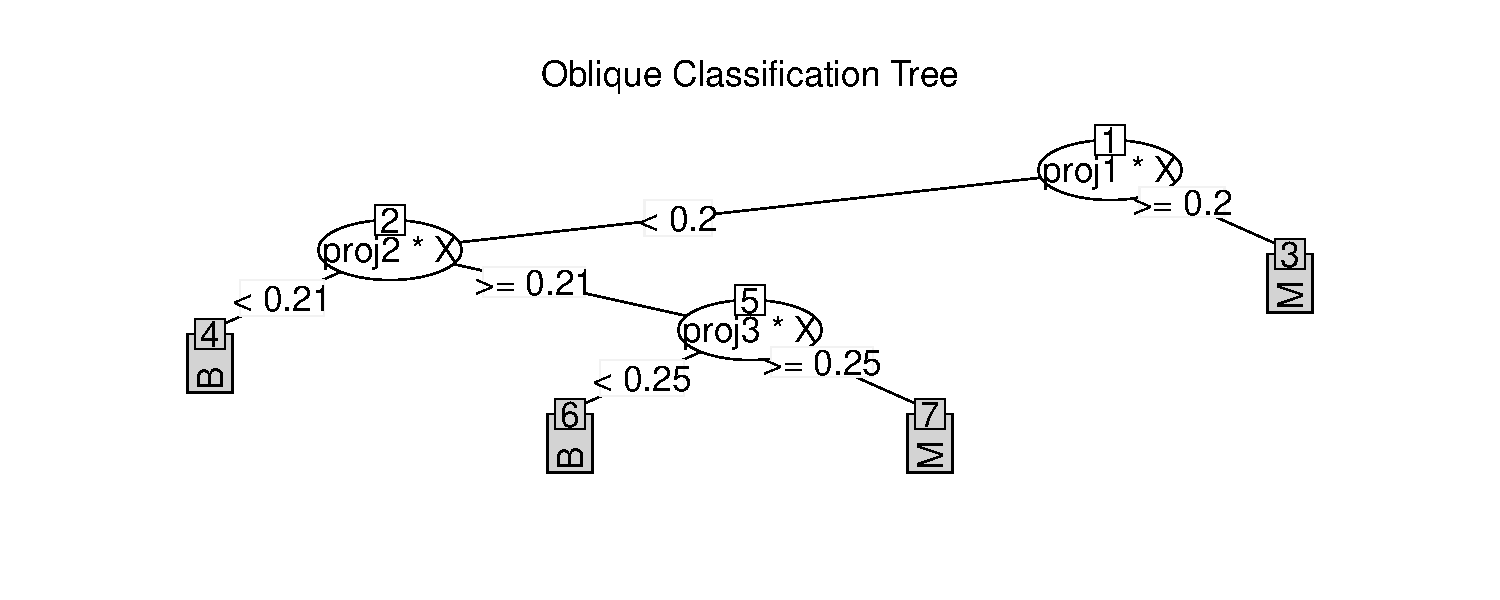
\includegraphics{ODRF-tree}
%%%%%%%%%%%%%%%%%%%%%%%%%%
\caption{\label{fig:cancer.tree} The ODT tree structure of breast cancer}
\end{figure}
\begin{table}[t!]
  \centering
    \begin{tabular}{lrrr}
    \toprule
    varibles & proj1 & proj2 & proj3 \\
    \midrule
    x3: perimeter\_mean & -0.434  & 0.000  & 0.000  \\
    x6: compactness\_mean & 0.000  & -0.571  & 0.000  \\
    x8: concave.points\_mean & -0.206  & 0.000  & 0.000  \\
    x9: symmetry\_mean & 0.000  & -0.275  & 0.000  \\
    x13: perimeter\_se & 0.000  & 0.413  & 0.000  \\
    x14: area\_se & 0.608  & 0.000  & 0.000  \\
    x21: radius\_worst & 0.486  & 0.000  & 0.000  \\
    x22: texture\_worst & 0.000  & 0.175  & 0.000  \\
    x23: perimeter\_worst & 0.000  & 0.000  & 1.000  \\
    x24: area\_worst & 0.000  & 0.153  & 0.000  \\
    x28: concave.points\_worst & 0.400  & 0.612  & 0.000  \\
    \bottomrule
    \end{tabular}%
    \caption{the projections of breast cancer}\label{tab:proj}%
\end{table}%
%% -- Summary/conclusions/discussion -------------------------------------------
%\section{Summary and discussion} \label{sec:summary}


%% -- Bibliography -------------------------------------------------------------
%% - References need to be provided in a .bib BibTeX database.
%% - All references should be made with \cite, \citet, \citep, \citealp etc.
%%   (and never hard-coded). See the FAQ for details.
%% - JSS-specific markup (\proglang, \pkg, \code) should be used in the .bib.
%% - Titles in the .bib should be in title case.
%% - DOIs should be included where available.

\bibliography{refs}

%% -----------------------------------------------------------------------------

\end{document}
